% !TeX root = Bericht.tex
% !TeX spellcheck = de_DE
\section{Theory}
\label{sec:theorie}
In this section, all necessary theoretical backgrounds are presented. Some theory belonging to spectroscopy is described as well as corrections of raw data frames.
\subsection{Spectroscopy}


When analysing absorption lines in a spectrum, the equivalent width of a line is determined. This width $EW$ is formally defined as 
\begin{equation}
	EW=\int \frac{I_0-I_\lambda}{I_0}d\lambda,
\end{equation}
where $I_0$ is the constant continuum intensity, and $I_\lambda$ is is the intensity measured at a certain wavelength $\lambda$. Graphically, the equivalent width can be described as the width of a square with length of the continuum intensity, as can be seen in \autoref{bild_linewidth}. The area of the square hereby has to equal the missing area of the absorption line. 

\begin{figure}[H]
	\centering
	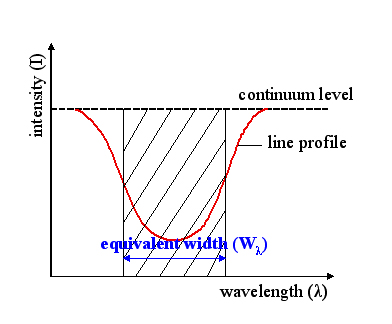
\includegraphics[width=0.5\textwidth]{Definition_of_equivalent_width}
	\caption{Visualization of the equivalent width of a line profile of an absorption line. Figure taken from \cite{bild_linewidth} }
	\label{bild_linewidth}
\end{figure}
The equivalent width depends on the number of atoms $N_i$ in an absorbing medium. The number of atoms $N_i$ is relative to a gas column with a certain volume. The behavior of the equivalent width dependent on $N_i$ is called the curve of growth. Atomic states are distributed via Boltzmann-distribution, leading to
\begin{equation}
	EW_\lambda=\frac{N_{r0}}{g_{r0}}g_{rs}f_{rs}\lambda^2 \exp{(-\chi_i/(k_{\mathrm{B}}T)}. \label{schwierig}
\end{equation}
Here, $f$ describes the oscillator strengths, $g$ the degeneracy, $r$ and $s$ are the quantum numbers of both levels involved in the transition. This approximation, however, is only valid for thin absorbing layers. Above the validity range of the approximation, saturation occurs. Doppler and Stark broadening are getting relevant here, and lead the curve of growth to a new regime \cite{spectroscopy}.
Based on \autoref{schwierig}, we can derive 
\begin{equation}\label{eqn:line}
	\log(EW_\lambda/\lambda)-\log(\lambda g f)=-\frac{5040}{T}\chi+\log(N_\mathrm{i}/N_\mathrm{H}). 
\end{equation}
Using this relation, the growth curve can be determined, using the equivalent width, wavelength and the factor $\log{(gf)}$. To receive this data, we are fitting a gaussian function to every peak. Out of the fit-parameters, we get the equivalent width and wavelength, the third factor is used from a table. 
\subsection{Echelle-spectrograph}
In order to get a spectrum out of light, we need to disperse the light. Therefore, in our case, an Echelle-spectrograph is used. This type of spectrograph offers high resolutions, meaning that it can resolve a large range of wavelengths. The intensity, in contrast, is very low for high resolutions, as the intensity is distributed on many orders, in contrast to focusing on only one specific order. 
A second grating with lower resolution is used after the first one, and disperses light perpendicular. Because of this setup, the spectra of individual orders are placed on top of each other in the resulting frame. As a result of the two gratings, the recorded spectra are curved, due to occuring nonlinear dispersion terms. 



%\begin{figure}[H]
%    \centering
%    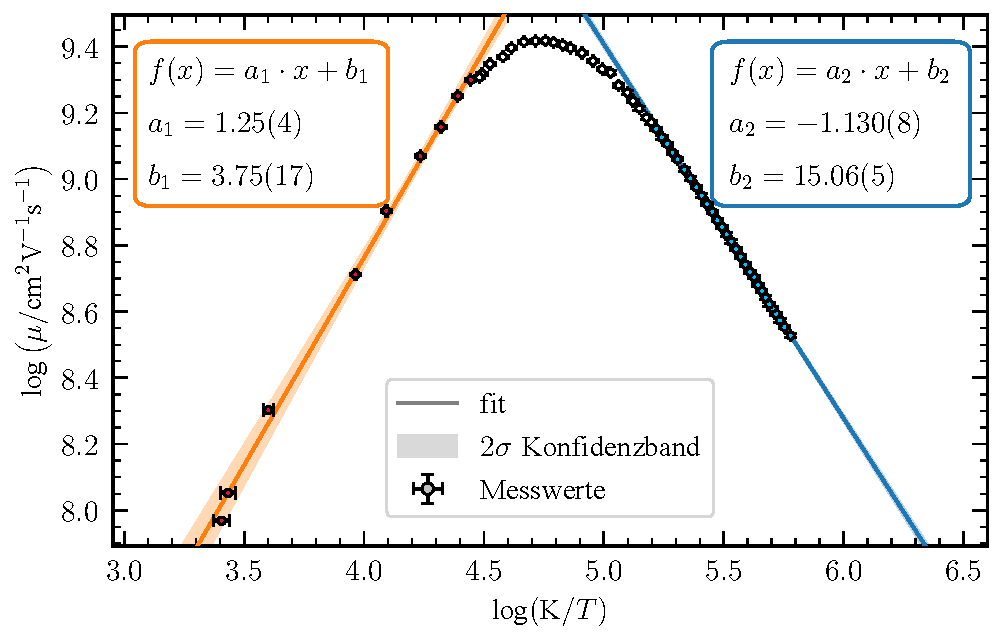
\includegraphics[width=\textwidth]{plot3.pdf}
%    \caption{}
%    \label{fig:plot3}
%\end{figure}


\subsection{Data processing}
In order to get a sun spectra of high quality, we need to process the raw data. Therefore, some important measurements and corrections have to be made. 
The first one of these is called the bias subtraction. It gets rid of signal that is recorded, while the sensor is not exposed to any light. Thus, the bias is a constant offset, which has to be subtracted from the raw file. The bias can be measured by taking pictures without exposing the CCD sensor to light. \newline

The second step is to do a flatfield correction. The CCD sensors sensitivity is not equal on the complete sensor. Therefore, the whole sensor is exposed uniformly to a light source, the sensors response then should be constant for a perfect sensor. Nevertheless, some deviations can be seen in these flatfield frames. To correct the raw data, the data frame has to be divided by an averaged flatfield frame.  \newline

As it is unknown which pixel on the CCD corresponds to which wavelength, a wavelength calibration needs to be carried out. To do so, the sensor is illuminated with a ThAr-lamp. The emitted wavelengths of this lamp is known, thus the pixels can be calibrated this way. 

After these three steps of correcting and calibrating, the two-dimensional frame needs to be converted to a one-dimensional spectrum. 

